\documentclass[serif, aspectratio=169]{beamer}
\usepackage[T1]{fontenc} 
\usepackage{fourier}
\usepackage{hyperref}
\usepackage{latexsym,amsmath,xcolor,multicol,booktabs,calligra}
\usepackage{booktabs} % For better table formatting
\usepackage{graphicx,pstricks,listings,stackengine}
\usepackage{listings}
\usepackage{array} 
\usepackage{colortbl}

\author{Dr.Hajialiasgari}
\title{Machine Learning}
\institute{
    Tehran University \\
    Of\\
    Medical Science
}
\date{\small \today}
\usepackage{UoWstyle}

% Define custom colors and styles for listings
\definecolor{deepblue}{rgb}{0,0,0.5}
\definecolor{deepred}{RGB}{153,0,0}
\definecolor{deepgreen}{rgb}{0,0.5,0}
\definecolor{halfgray}{gray}{0.55}

\lstset{
    basicstyle=\ttfamily\small,
    keywordstyle=\bfseries\color{deepblue},
    emphstyle=\ttfamily\color{deepred},
    stringstyle=\color{deepgreen},
    numbers=left,
    numberstyle=\small\color{halfgray},
    rulesepcolor=\color{red!20!green!20!blue!20},
    frame=shadowbox,
}

\begin{document}

\begin{frame}
    \titlepage
    \vspace*{-0.6cm}
    \begin{figure}[htpb]
        \begin{center}
            \includegraphics[keepaspectratio, scale=0.05]{Tumsl-logo.png}
        \end{center}
    \end{figure}
\end{frame}

\begin{frame}    
\tableofcontents[sectionstyle=show, subsectionstyle=show/shaded/hide, subsubsectionstyle=show/shaded/hide]
\end{frame}


\section{Boosting}

\subsection{Motivation and Baisc idea}

\begin{frame}{Boosting: Motivation}
    \begin{itemize}
        \item Many simple models (weak learners) have high bias and fail to capture complex patterns.
        \item Instead of training a single strong model, boosting improves weak models sequentially.
        \item Boosting minimizes errors by giving more importance (higher weights) to misclassified instances.
        \item It reduces bias and variance, making the model more accurate and robust.
    \end{itemize}
\end{frame}

\begin{frame}{Boosting: Basic Idea}
    \begin{enumerate}
        \item Train a weak learner (e.g., a shallow decision tree) on the dataset.
        \item Identify misclassified instances and assign them higher weights.
        \item Train the next weak learner, focusing more on these hard-to-classify samples.
        \item Repeat the process iteratively, combining all weak learners into a strong final model.
        \item Final prediction is made using a weighted combination of all weak learners.
    \end{enumerate}
\end{frame}


\begin{frame}{Basic idea (Cont.)}
    \centering
    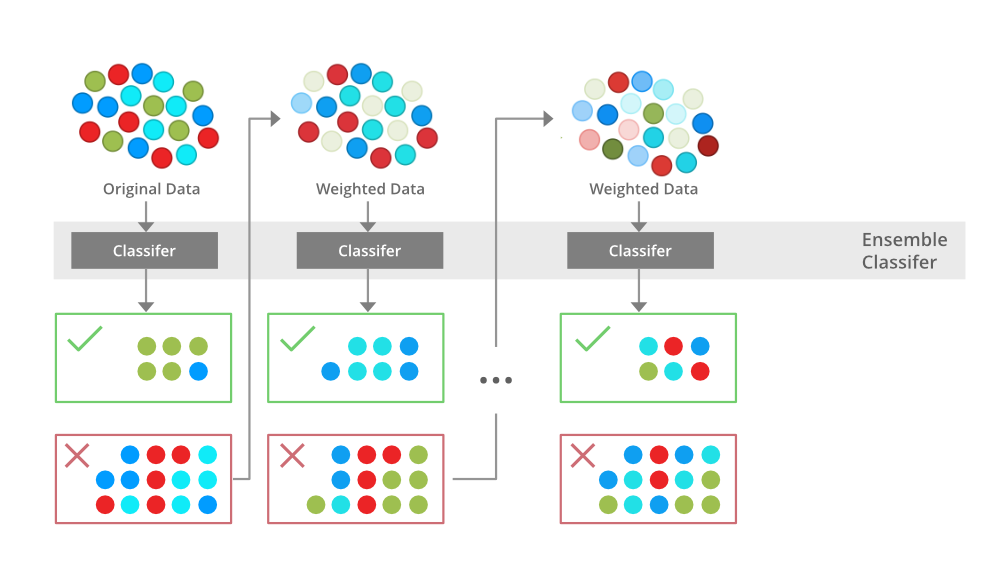
\includegraphics[width=0.9\textwidth]{Boosting.png}
\end{frame}

\begin{frame}{Popular Boosting Techniques}
    \begin{itemize}
        \item \textbf{AdaBoost} (Adaptive Boosting)
        \item \textbf{Gradient Boosting} (GBM)
        \item \textbf{XGBoost} (Extreme Gradient Boosting)
    \end{itemize}
\end{frame}

\subsection{Algorithm}

\begin{frame}{General Boosting Algorithm}
    \textbf{Step-by-Step Algorithm:}
    \begin{enumerate}
        \item \textbf{Initialize Weights:} Start with equal weights for all training samples.
        \item \textbf{Train a Weak Model:} Train a simple model (e.g., decision stump).
        \item \textbf{Calculate Error:} Measure model performance.
        \item \textbf{Update Model Strength:} Give more weight to better-performing models.
        \item \textbf{Adjust Sample Weights:} Increase weight for misclassified samples.
        \item \textbf{Repeat Steps 2-5} for multiple rounds.
        \item \textbf{Final Prediction:} Combine all models’ outputs with appropriate weights.
    \end{enumerate}
\end{frame}

\begin{frame}{Boosting Formula}
    \textbf{Model Weight Calculation:}
    \begin{equation}
        \alpha_t = \frac{1}{2} \ln \left( \frac{1 - e_t}{e_t} \right)
    \end{equation}
    where $e_t$ is the model's error.
    
    \textbf{Final Boosted Model:}
    \begin{equation}
        H(x) = \text{sign} \left( \sum_{t=1}^{T} \alpha_t h_t(x) \right)
    \end{equation}
    Each weak model $h_t(x)$ contributes to the final decision.
\end{frame}

\subsection{AdaBoost}

\begin{frame}{Overview}
\textbf{Concept:} AdaBoost combines weak classifiers to create a strong classifier by assigning higher weights to misclassified points in each iteration.
\end{frame}
\begin{frame}{Algorithm}
\begin{enumerate}
    \item Initialize equal weights for all training examples.
    \item Train a weak classifier on the dataset.
    \item Compute the classifier's error.
    \item Assign higher weight to misclassified examples.
    \item Train the next weak classifier with updated weights.
    \item Repeat for a predefined number of iterations.
    \item Final prediction is a weighted sum of weak classifiers.
\end{enumerate}
\end{frame}

\begin{frame}{Algorithm (Cont.)}
    
\textbf{Formula:}
\begin{equation}
    \alpha_t = \frac{1}{2} \ln \left( \frac{1 - \epsilon_t}{\epsilon_t} \right)
\end{equation}
\begin{equation}
    w_{t+1} = w_t e^{\alpha_t}
\end{equation}
\end{frame}
\begin{frame}{Advantages and Disadvantages}
\textbf{Advantages:}
\begin{itemize}
    \item Simple and effective.
    \item Works well with noisy data.
    \item Less prone to overfitting.
\end{itemize}

\textbf{Disadvantages:}
\begin{itemize}
    \item Sensitive to outliers.
    \item Weak classifiers must be chosen carefully.
\end{itemize}
\end{frame}

\subsection{Gradient Boosting}
\begin{frame}{Overview}
\textbf{Concept:} Gradient Boosting fits new models to the residual errors of previous models, minimizing the loss function using gradient descent.
\end{frame}
\begin{frame}{Algorithm}
    
\begin{enumerate}
    \item Initialize the model with a constant value (e.g., mean of target values).
    \item Compute residuals (errors) between actual and predicted values.
    \item Train a weak model on residuals.
    \item Update the predictions by adding the weak model’s weighted output.
    \item Repeat until the error is minimized.
\end{enumerate}
\end{frame}

\begin{frame}{Algorithm (Cont.)}
    
\textbf{Formula:}
\begin{equation}
    r_i = y_i - f_{t-1}(x_i)
\end{equation}
\begin{equation}
    f_t(x) = f_{t-1}(x) + \gamma h_t(x)
\end{equation}
\end{frame}

\begin{frame}{Advantages and Disadvantages}
    
\textbf{Advantages:}
\begin{itemize}
    \item Handles missing data well.
    \item Can model complex relationships.
    \item Works well for structured data.
\end{itemize}

\textbf{Disadvantages:}
\begin{itemize}
    \item Computationally expensive.
    \item Sensitive to hyperparameter tuning.
\end{itemize}
\end{frame}

\subsection{XGBoost}

\begin{frame}{Overview}
\textbf{Concept:} XGBoost is an optimized version of Gradient Boosting that improves speed and performance using parallelization and regularization.
\end{frame}

\begin{frame}{Features}
\textbf{Key Features:}
\begin{itemize}
    \item Regularization (L1 \& L2) to prevent overfitting.
    \item Parallel computation for efficiency.
    \item Handles missing values internally.
\end{itemize}
\end{frame}

\begin{frame}{Algorithm}

\textbf{Algorithm Enhancements:}
\begin{enumerate}
    \item Uses a regularized objective function:
    \begin{equation}
        L = \sum_{i} l(y_i, \hat{y}_i) + \lambda \sum_{j} \theta_j^2
    \end{equation}
    where $\lambda$ is the regularization term.
    \item Uses second-order approximation to optimize loss faster.
    \item Performs tree pruning to avoid overfitting.
\end{enumerate}
\end{frame}

\begin{frame}{Advantages and Disadvantages}
\textbf{Advantages:}
\begin{itemize}
    \item Faster than traditional boosting.
    \item Built-in regularization.
    \item Works well for both regression and classification.
\end{itemize}

\textbf{Disadvantages:}
\begin{itemize}
    \item More complex than AdaBoost and Gradient Boosting.
    \item Requires careful tuning.
\end{itemize}
\end{frame}

\section{Stacking}
\subsection{Introduction}
\begin{frame}{Stacking in Ensemble Learning}
    \textbf{Definition:} Stacking (Stacked Generalization) is an ensemble learning technique that combines multiple base models to improve predictive performance by training a meta-model on their outputs.
\end{frame}
\subsection{Overview}
\begin{frame}{Stacking Overview}
    \begin{itemize}
        \item Unlike bagging and boosting, stacking focuses on learning how to best combine multiple models.
        \item It consists of base models (weak learners) and a meta-model that integrates their predictions.
        \item The meta-model is trained on the outputs of base models to generate the final prediction.
    \end{itemize}
\end{frame}

\subsection{Basic Idea of How Stacking Works}
\begin{frame}{How Stacking Works}
    \begin{enumerate}
        \item Train multiple base models (e.g., Decision Trees, SVM, k-NN) on the training set.
        \item Each base model makes predictions on:
        \begin{itemize}
            \item The training set (used to train the meta-model).
            \item The test set (used for final evaluation).
        \end{itemize}
        \item Collect the predictions of base models as new features.
        \item Train a meta-model (e.g., logistic regression) on these new features.
        \item Use the trained meta-model to make the final prediction.
    \end{enumerate}
\end{frame}

\subsection{Advantages and Disadvantages}
\begin{frame}{Advantages}
    \begin{itemize}
        \item Can improve accuracy by leveraging multiple models.
        \item Reduces overfitting if base models are diverse.
        \item Works well with complex data.
    \end{itemize}
\end{frame}

    
\begin{frame}{Disadvantages}
    \begin{itemize}
        \item Computationally expensive due to multiple model training.
        \item Requires careful selection of base models and meta-models.
        \item More complex compared to bagging and boosting.
    \end{itemize}
\end{frame}

\section{Comparison}

\begin{frame}{Comparison of Ensemble Methods (Part 1)}
    \centering
    \renewcommand{\arraystretch}{1.2} % Adjust row spacing for readability
    \begin{tabular}{|p{2cm}|p{2cm}|p{3cm}|p{4cm}|}
        \hline
        \textbf{Method} & \textbf{Type} & \textbf{Base Models} & \textbf{Combination Strategy} \\
        \hline
        Bagging & Parallel & Decision Trees, k-NN, etc. & Averaging / Majority Voting \\
        \hline
        Random Forest & Parallel & Decision Trees & Majority Voting / Averaging \\
        \hline
        Boosting & Sequential & Decision Trees (weak learners) & Weighted combination \\
        \hline
        AdaBoost & Sequential & Weak classifiers (e.g., Decision Stumps) & Weighted voting \\
        \hline
    \end{tabular}
\end{frame}

\begin{frame}{Comparison of Ensemble Methods (Part 2)}
    \centering
    \renewcommand{\arraystretch}{1.2} % Keep row spacing consistent
    \begin{tabular}{|p{2cm}|p{3cm}|p{4cm}|p{4cm}|}
        \hline
        \textbf{Method} & \textbf{Strengths} & \textbf{Weaknesses} \\
        \hline
        Bagging & Reduces variance, prevents overfitting & Less effective for high-bias models \\
        \hline
        Random Forest & Handles high-dimensional data, reduces overfitting & Computationally expensive with many trees \\
        \hline
        Boosting & Improves accuracy, reduces bias & Prone to overfitting if not regularized \\
        \hline
        AdaBoost & Focuses on hard-to-classify instances & Sensitive to noise and outliers \\
        \hline
    \end{tabular}
\end{frame}

\begin{frame}{Comparison of Ensemble Methods (Part 3)}
    \centering
    \renewcommand{\arraystretch}{1.2} % Keep row spacing consistent
    \begin{tabular}{|p{2cm}|p{2cm}|p{3cm}|p{4cm}|}
        \hline
        \textbf{Method} & \textbf{Type} & \textbf{Base Models} & \textbf{Combination Strategy} \\
        \hline
        Gradient Boosting & Sequential & Decision Trees & Gradient Descent Optimization \\
        \hline
        XGBoost & Sequential & Decision Trees & Gradient-based boosting with regularization \\
        \hline
        Stacking & Hybrid & Any ML models & Meta-learner combines predictions \\
        \hline
    \end{tabular}
\end{frame}

\begin{frame}{Comparison of Ensemble Methods (Part 4)}
    \centering
    \renewcommand{\arraystretch}{1.2} % Keep row spacing consistent
    \begin{tabular}{|p{2cm}|p{3cm}|p{4cm}|p{4cm}|}
        \hline
        \textbf{Method} & \textbf{Strengths} & \textbf{Weaknesses} \\
        \hline
        Gradient Boosting & Highly accurate, works well with complex data & Computationally expensive \\
        \hline
        XGBoost & Faster than Gradient Boosting, handles missing data & Requires careful tuning \\
        \hline
        Stacking & Leverages multiple models, improves performance & Computationally expensive, requires careful selection \\
        \hline
    \end{tabular}
\end{frame}


\begin{frame}
    \begin{center}
        {\Huge\ \color{red}For more information and code check the related notebook}
    \end{center}
\end{frame}

\begin{frame}
    \begin{center}
        {\Huge\ End of Ensemble Learning Part 2}
    \end{center}
\end{frame}

\end{document}

